\documentclass{beamer}
\usetheme{Gelugor}
\usepackage{hyperref}
\usepackage[utf8]{inputenc}
\usepackage[spanish]{babel}
\usepackage[default]{droidserif}
\title{Análisis y Diseño de Software}
\subtitle{Introducción a GitHub}
\author[Grupo1]{
Martha Suntaxi\\Johanna Paz\\Victor Jumbo\\Andre Montoya\\Wilson Iriarte
}
\date{\today}
\institute{Ingeniería en Sistemas\\}

\begin{document}
	
	%INICIO carátula
	\begin{frame}[plain,t]
		\titlepage
	\end{frame}
	%FIN carátula

	\section{Introducción a GitHub}

\subsection{Agenda}
\begin{frame}
\frametitle{Agenda}
{\small
\begin{itemize}
\item Introducción
	\begin{itemize}
	\item ¿Qué es GitHub?
	\item ¿Para que sirve?
	\item ¿Qué uso le daremos?
	\item ¿Qué herramientas proporciona?
	\end{itemize}
\item Git
	\begin{itemize}
	\item Mas sobre Git
	\item Los entresijos internos de Git
	\item Colaborar varias personas en un mismo Github
	\end{itemize}
\item Comandos Principales
	\begin{itemize}
	\item Comandos Básicos
	\item Trabajos con Ramas
	\item Acciones con Archivos
	\end{itemize}
\item Conclusiones
\end{itemize}}
\end{frame}
\subsection{Introducción}
		\begin{frame}
			\frametitle{Introducción}
			%\framesubtitle{Tema}
			\begin{center}
\includegraphics[width=2cm, height=3cm]{git.jpg}\end{center}
			\begin{center}\textbf{\Large ¿Qué es GitHub?}\end{center}
			GitHub es una plataforma de desarrollo colaborativo de software para alojar proyectos utilizando el 						sistema de control de versiones Git.\\
		\end{frame}
		\begin{frame}
			\frametitle{Introducción}
			%\framesubtitle{Tema}
			\begin{center}\textbf{\Large ¿Para que sirve?}\end{center}
			{\small \begin{itemize}
			\item Aloja tu repositorio de código y te brinda herramientas muy útiles para el trabajo en equipo, dentro 			de un proyecto.
			\item Se Puede contribuir a mejorar el software de los demás. Para poder alcanzar esta meta, GitHub provee 			de funcionalidades para hacer un fork y solicitar pulls.
			\end{itemize}\ \\
			Realizar un fork es simplemente clonar un repositorio ajeno (genera una copia en tu 						cuenta), para eliminar 	algún bug o modificar cosas de él. Una vez realizadas tus modificaciones puedes 					enviar un pull al dueño del proyecto. Éste podrá analizar los cambios que has realizado fácilmente, y si 				considera interesante tu contribución, adjuntarlo con el repositorio original.}
			\\
		\end{frame}
		\begin{frame}
			\frametitle{Introducción}
			%\framesubtitle{Tema}
			\begin{center}\textbf{\Large ¿Qué uso le daremos?}\end{center}
			{\small En nuestra especialidad “Programación”, fuimos aprendiendo cosas y creando programas de 							código abierto, fomentando el software libre.
			Podremos crear una cuenta gratuita y comenzar a subir repositorios de código (o crearlos desde 0), para 					que con la ayuda de todos ese proyecto mejore; así como también fortalecer los proyectos de los demás para 			crecer como grupo.}
		\end{frame}
		\begin{frame}
			\frametitle{Introducción}
			%\framesubtitle{Tema}
			\begin{center}\textbf{\Large ¿Qué herramientas proporciona?}\end{center}
			{\small En la actualidad, GitHub es mucho más que un servicio de alojamiento de código. Además de éste, se 			ofrecen varias herramientas útiles para el trabajo en equipo. Entre ellas, caben destacar:}
			{\footnotesize
			\begin{itemize}
			\item Una wiki para el mantenimiento de las distintas versiones de las páginas.
			\item Un sistema de seguimiento de problemas que permiten a los miembros de tu equipo detallar un problema 			con tu software o una sugerencia que deseen hacer.
			\item Una herramienta de revisión de código, donde se pueden añadir anotaciones en cualquier punto de un 				fichero y debatir sobre determinados cambios realizados en un commit específico.
			\item Un visor de ramas donde se pueden comparar los progresos realizados en las distintas ramas de 						nuestro repositorio.
			\end{itemize}}
		\end{frame}
\subsection{Git}
	\begin{frame}
		\frametitle{Git}
		%\framesubtitle{Tema}
		\begin{center}\textbf{\Large GIT - SOFTWARE DE CONTROL DE VERSIONES}\end{center}\\
		\\
		\begin{center}
			
\includegraphics[width=3cm,height=2cm]{gitlogo.jpg}
		\end{center}
		{\small
			\begin{itemize}
				\item {¿Qué es un software de control de versiones?}
				\item {¿Por qué git sobre otros software de control de versiones?}
				\item {¿Hay mas hostings que soporten git?}
			\end{itemize}
		}
	\end{frame}
	\begin{frame}
		\frametitle{Git}
		\framesubtitle{¿Qué es un software de control de versiones?}
		El control de versiones es un sistema que registra los cambios realizados sobre un archivo o conjunto de 				archivos a lo largo del tiempo, de modo que puedas recuperar versiones específicas más adelante. 
		\\
		\begin{center}
			
\includegraphics[width=2cm,height=3cm]{pregunta.jpg}
		\end{center}
	\end{frame}
	\begin{frame}
		\frametitle{Git}
		\framesubtitle{¿Por qué git sobre otros software de control de versiones?}
		\begin{itemize}	
			\item Fácil de usar.
			\item Rápido y eficiente en grandes proyectos
			\item Sistema de ramificación (branching) para desarrollo no lineal.
		\end{itemize}
	\end{frame}
	\begin{frame}
		\frametitle{Git}
		\framesubtitle{¿Hay mas hostings que soporten git?}
		\begin{itemize}	
			\item Google Code.
			\item Gforce
			\item Assembla
		\end{itemize}
	\end{frame}
	\begin{frame}
		\frametitle{Mas sobre Git}
		\textbf{ Modelado de datos en Git.}\\
		\begin{center}
			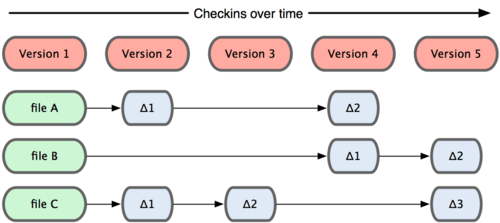
\includegraphics[width=6cm,height=4cm]{imagen1.png}
		\end{center}
	\end{frame}

	\begin{frame}
		\frametitle{Mas sobre Git}
		\textbf{Git modela sus datos más como un conjunto de instantáneas de un mini sistema de archivos.}\\
		\begin{center}
			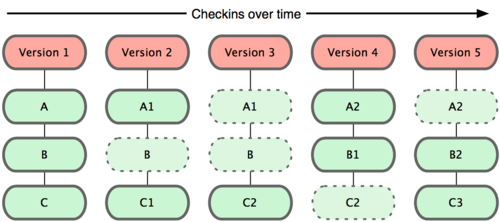
\includegraphics[width=6cm,height=4cm]{imagentxt.png}
		\end{center}
	\end{frame}	

	\begin{frame}
		\frametitle{Mas sobre Git}
		\begin{itemize}	
			\item \textbf{Casi cualquier operación es local}
				\begin{itemize}	
					\item No se necesita información
					\item Historia del proyecto
					\item No conexión
				\end{itemize}
			\item \textbf{Tiene integridad}
				\begin{itemize}	
					\item Todo en Git es verificado
					\item Si git no lo sabe
					\item El valor hash de git
				\end{itemize}
			\item \textbf{Generalmente sólo añade información}
		\end{itemize}
		{\scriptsize \textbf{Nota: } El mecanismo de comprobación de git se conoce como hash SHA-1 y es asi: 
		\\{\tt  24b9da6552252987aa493b52f8696cd6d3b00373}}\\
	\end{frame}
	
	\begin{frame}
		\frametitle{Mas sobre Git}
		\textbf{Los tres estados.}\\
		\begin{itemize}		
			\item Confirmado
			\item Modificado
			\item Preparado
		\end{itemize}
		\begin{center}
			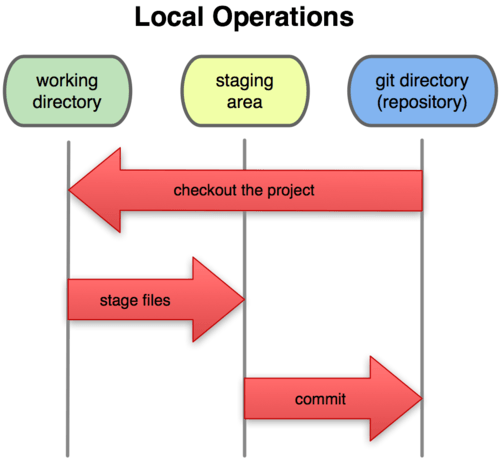
\includegraphics[width=4cm,height=5cm]{imagen3.png}
		\end{center}
	\end{frame}

	\begin{frame}
		\frametitle{Los entresijos internos de Git}
		\begin{itemize}
			\item ¿Qué pasa cuando lanzas 'git init'?.\\
		\end{itemize}
		\begin{center}
			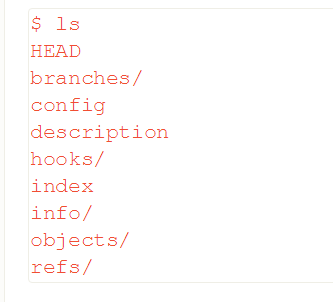
\includegraphics[width=5cm,height=4cm]{imagen4.png}
		\end{center}
	\end{frame}

	\begin{frame}
		\frametitle{Los entresijos internos de Git}
		\textbf{Los objetos Git}\\
		Git es un sistema de archivo orientado a contenidos. Estupendo. Y eso, ¿qué significa?\\
	\end{frame}
	\begin{frame}
		\frametitle{Los entresijos internos de Git}
		\framesubtitle{Obteniendo un repositorio Git}
		\begin{itemize}	
			\item Inicializando un repositorio en un directorio existente
			{\tt  git add}
			\item Clonando un repositorio existente
			{\tt  git clone[url]}
			\item Sistema de ramificación (branching) para desarrollo no lineal.
		\end{itemize}
	\end{frame}
	\begin{frame}
		\frametitle{Los entresijos internos de Git}
		\framesubtitle{Guardando cambios en el repositorio}
		Recuerda que cada archivo de tu directorio de trabajo puede estar en uno de estos dos estados: 
		\begin{itemize}
			\item Bajo seguimiento (tracked). 
			\item Sin seguimiento (untracked).
		\end{itemize}
		\begin{center}
			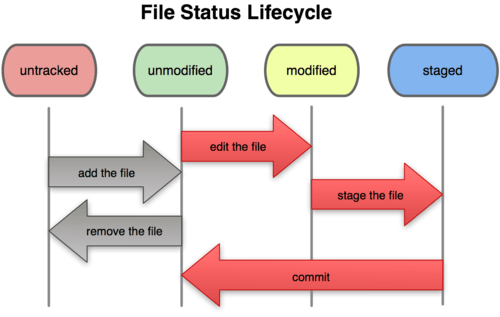
\includegraphics[width=5cm,height=3cm]{imagen5.png}
		\end{center}
	\end{frame}
	\begin{frame}
		\frametitle{Los entresijos internos de Git}
		\textbf{\small Comprobando el estado de tus archivos}
		\begin{center}
			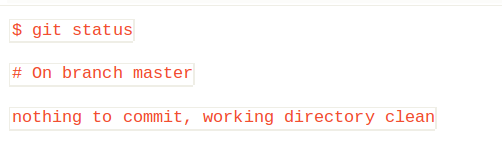
\includegraphics[width=5cm,height=2cm]{captura1.png}
		\end{center}
		\textbf{\small Al añadir un nuevo archivo a tu proyecto}
		\begin{center}
			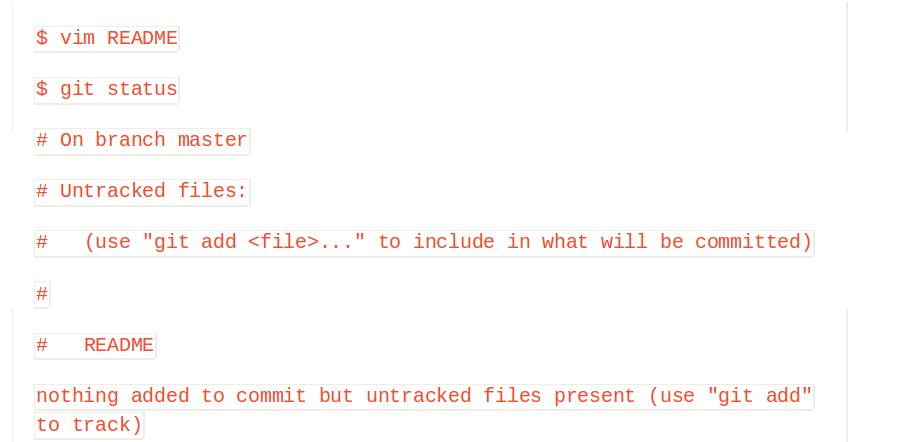
\includegraphics[width=5cm,height=3cm]{captura2.png}
		\end{center}
	\end{frame}
	\begin{frame}
		\frametitle{Los entresijos internos de Git}
		\textbf{Retornar a una version anterior}\\
		La base de datos contendrá todas versiones del archivo
		\\
		{\tt\scriptsize \$ find .git/objects -type f 
.git/objects/1f/7a7a472abf3dd9643fd615f6da379c4acb3e3a
.git/objects/83/baae61804e65cc73a7201a7252750c76066a30
.git/objects/d6/70460b4b4aece5915caf5c68d12f560a9fe3e4}
		\\		
		Para revertir el archivo a su primera versión:\\
		{\tt\scriptsize \$ git cat-file -p 83baae61804e65cc73a7201a7252750c76066a30}
	\end{frame}
	\begin{frame}
		\frametitle{Los entresijos internos de Git}
		\textbf{Preparando archivos modificados}
		Esto significa que un archivo bajo seguimiento ha sido modificado en el directorio de trabajo, pero no ha sido preparado todavía, Para prepararlo, ejecuta el comando \\
		{\tt git add}\\
	\end{frame}
	\begin{frame}
		\frametitle{Los entresijos internos de Git}
		\textbf{Confirmando tus cambios}
		Puedes confirmar los cambios escribiendo \\
		{\tt git commit}\\
		Podemos anadir la opción –v(se añadan también las diferencias de tus cambios) o –m( escribir tu mensaje de confirmación)
		\begin{itemize}
			\item –v Se añaden las diferencias de tus cambios
			\item –m Escribir tu mensaje de confirmación
		\end{itemize}
	\end{frame}
	
	\begin{frame}
		\frametitle{Los entresijos internos de Git}
		\textbf{Enviando a tus repositorios remotos}
		{\tt git push [nombre-remoto][nombre-rama]}\\
		Este comando funciona únicamente si has clonado de un servidor en el que tienes permiso de escritura, y nadie ha enviado información mientras tanto. 
	\end{frame}
	\begin{frame}
		\frametitle{¿Si tú y otra persona clonan a la vez, y él envía su información y luego envías tú?}
		Pues sencillamente quien llegue de segundo será rechazado.
		\\[8]
		\textbf{Nota: } Si desean profundizar mas en el tema la guía de git en el capítulo 9 tiene mas información.
	\end{frame}	
	\begin{frame}
		\frametitle{Colaborar varias personas en un mismo Github}
		\begin{itemize}
			\item ¿Cómo resuelve git el problema?
			\item ¿Para qué sirve hacer un Fork?
			\item ¿Qué ventajas trae este proceso?
		\end{itemize}
	\end{frame}	

\subsection{Comandos}
	\begin{frame}
		\frametitle{Comandos Básicos}
		\begin{itemize}
			\item Inicializar repositorio git
			\begin{center}
				 {\tt \scriptsize git init}\\
			\end{center}
			\item Creación de un fichero README 
			\begin{center}
				 {\tt \scriptsize vi README.md}\\
			\end{center}
			\item Añadir a Git los ficheros modificados.
			\begin{center}
				 {\tt \scriptsize git add README.md}\\	 
			\end{center}
			\item Enviar los cambios hacia GitHub
			\begin{center}
				 {\tt \scriptsize git push origin master}\\	 
			\end{center}
		\end{itemize}
	\end{frame}
	\begin{frame}
		\frametitle{Ramas}
		Las ramas son utilizadas para desarrollar funcionalidades aisladas unas de otras.
		\begin{itemize}
			\item Crear una rama
			\begin{center}
				 {\tt \scriptsize git branch <nombre rama>}\\
			\end{center}
			\item Cambiar de rama
			\begin{center}
				 {\tt \scriptsize git checkout <nombre rama>}\\
			\end{center}
			\item Eliminar una rama
			\begin{center}
				 {\tt \scriptsize git branch -d <nombre rama>}\\	 
			\end{center}
			\item Renombrar una rama
			\begin{center}
				 {\tt \scriptsize git branch -m <vieja rama> <nueva rama>}\\	 
			\end{center}
		\end{itemize}
	\end{frame}
	\begin{frame}
		\frametitle{Acciones con Archivos}
		\begin{itemize}
			\item \textbf{Deshacer cambios locales (reset)}: Con este comando descartamos los cambios locales y volvemos al estado que teníamos guardado en el respositorio
			\begin{center}
				 {\tt \scriptsize git reset --hard}\\
			\end{center}
			\item Desahacer los cambios realizados en todos los archivos
			\begin{center}
				 {\tt \scriptsize git checkout -- .}\\
			\end{center}
			\item Actualizar repositorio local
			\begin{center}
				 {\tt \scriptsize git pull}\\	 
			\end{center}
			\item Fusionar ramas
			\begin{center}
				 {\tt \scriptsize git merge <branch>}\\	 
			\end{center}
			\item Crear una nueva etiqueta en este caso se llama 1.0.0
			\begin{center}
				 {\tt \scriptsize git tag 1.0.0 1b2e1d63ff}\\	 
			\end{center}
			\item Obtener el commit id
			\begin{center}
				 {\tt \scriptsize git log}\\	 
			\end{center}
		\end{itemize}
	\end{frame}

\subsection{Conclusiones}
\begin{frame}
\frametitle{Conclusiones}
	\begin{itemize}
			\item Es un excelente repositorio para el desrrollo en grupo.
			\item Podemos obtener conocimientos gracias a que es un repositorio donde se encuentra codigo profesional de manera gratuita.
			\item Podemos colaborar con el crecimeinto de sofware libre, subiendo nuestros codigos al repositorio.
		\end{itemize}
\end{frame}

\subsection{Bibliografía}
\begin{frame}
\frametitle{Bibliografia}
	\begin{enumerate}
		\item L. Castillo, Conociendo GitHub. \url{https://conociendogithub.readthedocs.org/en/latest/}.
		\item Y. Torregrosa, Álvaro.Luján Mora, Sergio,2013 \url{http://rua.ua.es/dspace/handle/10045/26796}.
		\item Ruiz, José Arístides Valencia.Revista San Gregorio,2015 \url{http://revista.sangregorio.edu.ec/index.php/RSANG/article/view/66}.
	\end{enumerate}
\end{frame}

\subsection{Licencia}
\begin{frame}
\frametitle{Licencia}
\begin{center}
\href{http://www.google.com}{
\includegraphics[scale=.8]{cc}}
\end{center}
\end{frame}

\MuchasGraciasFrame

\end{document}
